\section{Постановка задачи}
	Начальная скорость на входе в канал $U_0 = 0.29$ м/с.
	На выходе из канала выставлено условие равенства нулю производной по нормали к границе.
	\begin{equation}
		\frac{\partial}{\partial n} = 0
	\end{equation}
	Граничные условия непротекания и прилипания устанавливаются для стенки. Это выражено равенством нулю нормальной и тангенциальной составляющих скорости.
	\begin{equation}
		v \cdot n = 0 \qquad v \cdot \tau = 0
	\end{equation}
	Здесь $n$ и $\tau$ представляют собой единичные векторы нормали и касательной к поверхности канала. Граничные условия для давления выставляются при помощи дискретизации уравнения изменения количества движения в проекции на нормаль к стенке.

\section{Визуализация поставленной задачи}
	Для построения геометрии канала и создания сеточной модели использовались встроенные средства по ANSYS.
\subsection{Геометрия канала}
	Объектом исследования является турбулентный пограничный слой в канале. Канал разбит на две части. Первая часть представляет собой сужение от 369.5$\times$149.8 мм в начале до размеров 124$\times$50 мм. Длина этого участка 396 мм. Он позволяет значительно увеличить скорость потока жидкости. Вторая часть -- прямолинейная, длиною в 1100 мм.
	\begin{figure}[H]
		\centering
		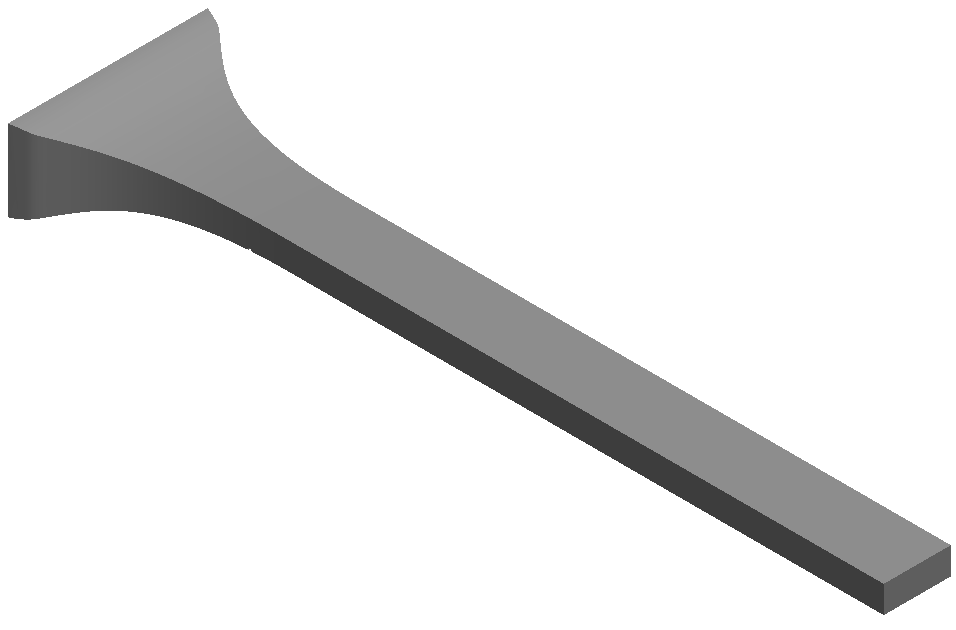
\includegraphics[width=0.7\linewidth]{../Assets/ВидКанала1}
		\caption{Общий вид канала}
		\label{fig:channelview}
	\end{figure}
	На расстоянии 323.9 мм от входа в канал, у основания расположен вырез представляющий проволоку радиусом 2.1 мм и высотой 1.98 мм. Это препятствие и создаёт турбулентное состояние. 
	\begin{figure}[H]
		\centering
		
\includegraphics[width=0.6\linewidth]{../Assets/ВидКанала4}
		\caption{Вид препятствия в канале}
		\label{fig:vortexgeneratorview}
	\end{figure}

\subsection{Построение сеточной модели}
	% Описать построение сетки, способы и про оптимизацию + схема из отчёта + вся статистика сетки %
	Существует несколько методов моделирования сеточных моделей в Ansys, которые можно использовать в зависимости от типа и размера модели.
	
	Первый -- это метод пространственного разбиения, который часто используется для моделирования твердых тел. Этот метод заключается в разбиении объекта на более мелкие элементы, называемые конечными элементами. Затем каждый конечный элемент аппроксимируется более простыми формами, такими как треугольники или прямоугольники, чтобы создать сетку.
	
	Второй -- это метод генерации сетки на основе узлов. В этом методе модель представляется в виде набора узлов, соединенных линиями или поверхностями. Затем сетка строится на основе этой структуры.
	
	Третий -- это метод многократного разделения. Этот метод часто используется для моделирования пространственных объектов, таких как воздушные суда или автомобили. Он заключается в разбиении объекта на более мелкие блоки и последующем разделении каждого блока на еще более мелкие блоки. Затем каждый блок аппроксимируется более простыми формами для создания сетки.
	
	\begin{figure}[H]
		\centering
		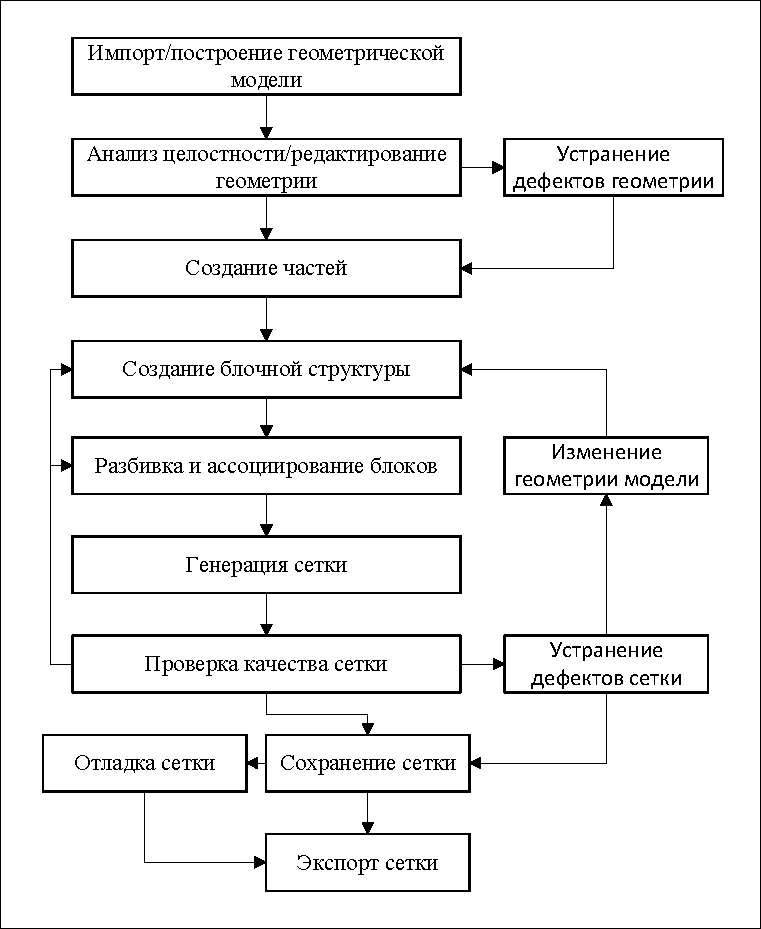
\includegraphics[width=0.8\linewidth]{../Assets/СхемаСозданияСеткиRU}
		\caption{Схема работы над сеточной моделью}
		\label{fig:meshScheme}
	\end{figure}
	
	На рисунке \ref{fig:meshScheme} представлена схематический план генерации сетки. Этот способ наиболее оптимальный для построения достаточно качественной сеточной модели. Разбиение геометрии на части позволяет ускорить построение, путём параллельного распределения вычислений(на каждую часть выделяется одно ядро). Кроме того, выключения режима многопоточности(одно физическое ядро делится на два виртуальных) для процессора увеличивает производительность, т. к. используется вся мощность ядра, а не его половина.
	
	% Перефразировать этот абзац и более красивее и обьёмнее + нужны хорошие скриншоты сетки %
	В результате работы над сеточной моделью удалось добиться оптимального результата для вычислений. Модель канала была разбита на 4 блока. Первый блок -- вход в канал, второй -- участок с препятствием, третий -- до конца сужения, четвёртый -- прямой участок канала. Статистика сетки: 51397337 узлов и 12665608 элементов. Полученная модель имеет уплотнение к низу канала, т. к. особую важность для изучения в данной работе составляет пограничный слой.
	\begin{figure}[H]
		\centering
		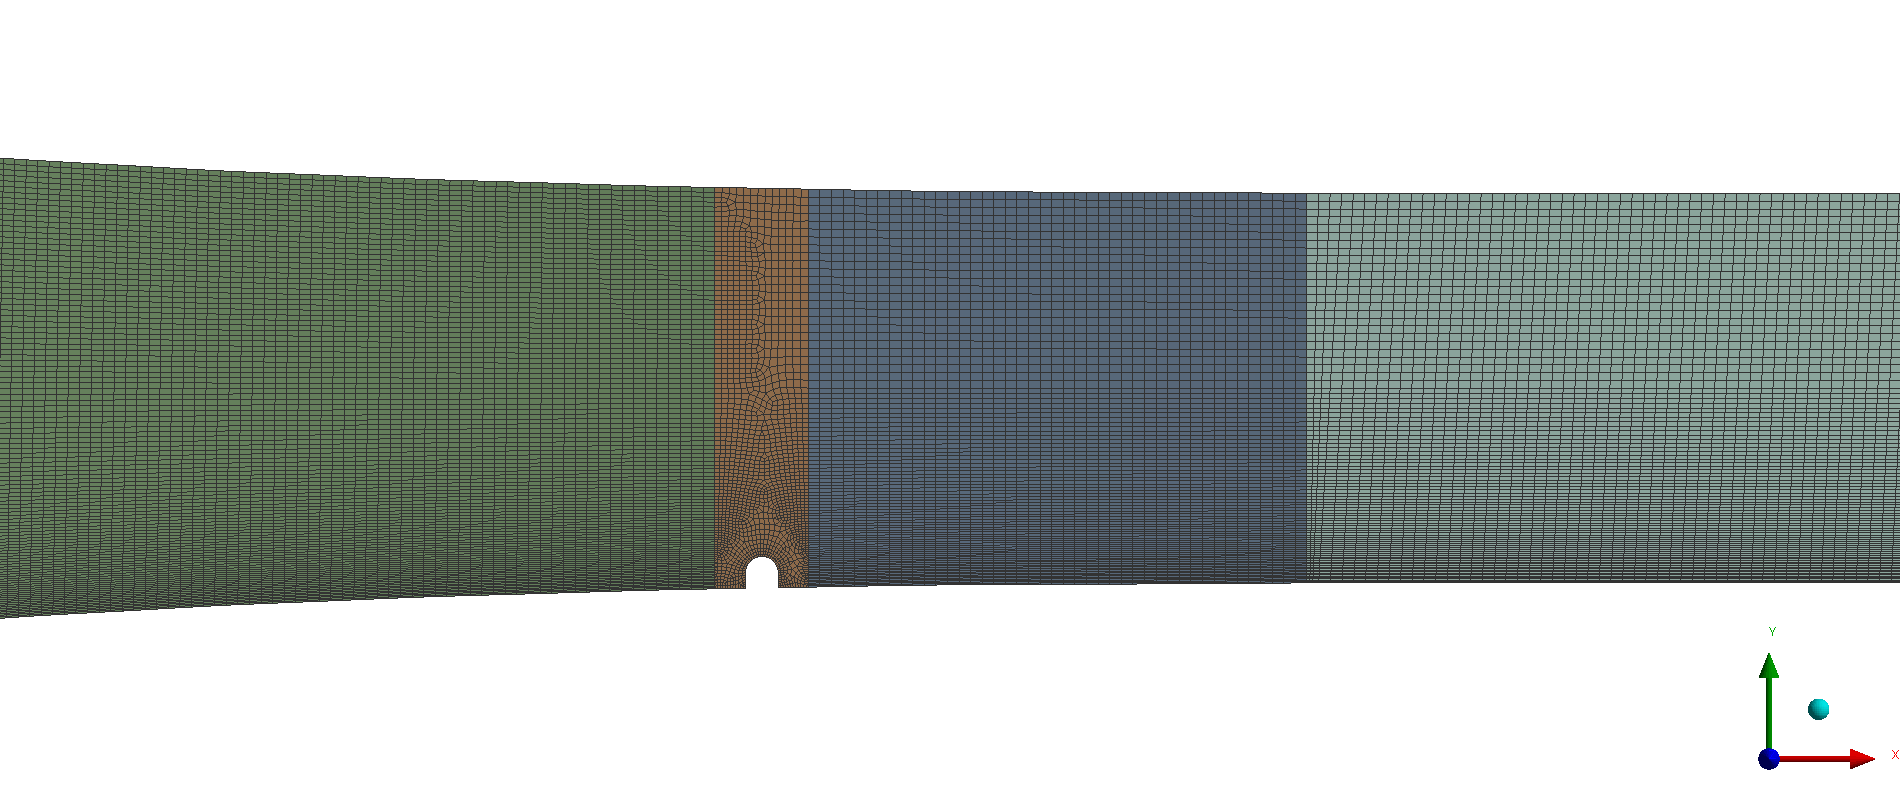
\includegraphics[width=1\linewidth]{../Assets/Mesh1}
		\caption{Сеточная модель}
		\label{fig:mesh1}
	\end{figure}
	
\section{Вычисление в ANSYS Fluent}
	% ???тензор??? %
	ANSYS Fluent -- это программное обеспечение для численного моделирования физических процессов в жидкостях, газах и теплообменных устройствах. С помощью ANSYS Fluent можно проводить расчеты течения жидкости или газа, теплопередачи, химических реакций и других важных явлений. Программа поддерживает широкий спектр физических моделей и методов решения, что позволяет ее применять для самых разнообразных задач. ANSYS Fluent имеет удобный пользовательский интерфейс, который позволяет легко создавать, настраивать и запускать вычислительные модели. Также программа предоставляет мощные инструменты для анализа результатов и визуализации данных. В целом, ANSYS Fluent является одной из самых популярных и мощных программ для численного моделирования в области тепло- и массопереноса, гидродинамики и других областей физики.
	
	В качестве жидкости использовалась вода c характеристиками: $\rho = 998.2$ $kg/m^3$ и $\nu = 0.001003$ $kg/m\cdot s$. Для подсеточной модели метода LES использовалась модель WALE c коэффициентом $C_w = 0.325$. Основные преимущества данной модели:
	\begin{itemize}
		\item пространственный оператор содержит как локальные деформации, так и скорости вращения. Таким образом, все структуры турбулентности, имеющие отношение к диссипации кинетической энергии, вычисляются этой моделью;
		\item турбулентная вязкость естественным образом стремится к нулю вблизи стенки, так что ни постоянная(динамическая) регулировка, ни функция демпфирования не требуются для расчета течений, ограниченных стенкой;
		\item модель дает нулевую турбулентную вязкость при чистом сдвиге. Таким образом, он может воспроизвести процесс перехода от ламинарного к турбулентному потоку за счет роста линейных неустойчивых режимов. 
	\end{itemize}
	Кроме того, модель WALE инвариантна к любому перемещению или вращению координат, и требуется только локальная информация (отсутствие операции проверки-фильтрации и сведений о ближайших точках в сетке), так что она хорошо подходит для LES в сложных геометриях\cite{Nicoud1999}.
	
	Параметры, связанные с расчётом уравнений:
	\begin{table}[H]
		\begin{center}
			\begin{tabular}{|c|c|}
				\hline
				Параметр & Метод\\
				\hline
				Схема & SIMPLEC \\
				\hline
				Градиент & Least squares cell based\\
				\hline
				Давление & Second order\\
				\hline
				Импульс & Bounded central differencing\\
				\hline
				Время & Bounded second order implicit\\
				\hline
			\end{tabular}
		\end{center}
		\caption{Перечень параметров решателя}
	\end{table}
	
	С описанными настройками и параметрами выше, был запущен расчёт в ANSYS FLUENT. Размер временного шага $\Delta t = 0.001 s$, их количество $s_t = 10000$. На каждый шаг рассчитывалось $s_i = 50$ итераций. Это составляет 10 с реального времени.